%
% Master thesis template for Ghent University (2021)
%
%
%  !!!!!!!!!!!!!!!!!!!!!!!!!!!!!!!!!!!!!!!!!!!!!!!!!!!!!!!!!!!!
%  !!        MAKE SURE TO SET XeLaTex AS LATEX ENGINE        !!
%  !!!!!!!!!!!!!!!!!!!!!!!!!!!!!!!!!!!!!!!!!!!!!!!!!!!!!!!!!!!!
%  !! For overleaf:                                          !!
%  !!     1. click gear icon in top right                    !!
%  !!     2. select `XeLaTex` in "latex engine"              !!
%  !!     3. click "save project settings"                   !!
%  !!                                                        !!
%  !!!!!!!!!!!!!!!!!!!!!!!!!!!!!!!!!!!!!!!!!!!!!!!!!!!!!!!!!!!!
%
%
%  History
%    2014         Doctoral Thesis of Bruno Volckaert
%    2017         Adapted to master thesis by Jerico Moeyersons
%    2018         Cleanup by Merlijn Sebrechts
%    2021         Update by Marleen Denert and Merlijn Sebrechts with feedback from Leen Pollefliet
%    2022         Update by Merlijn Sebrechts
%
%  Latest version
%    https://github.com/galgalesh/masterproef-template
%

% Note: remove `openany` for printed version
\documentclass[11pt,a4paper,openany,dutch,english]{book}
\usepackage[a4paper,includeheadfoot,margin=2.50cm]{geometry}




\renewcommand{\baselinestretch}{1.2}  % stretch horizontal space between everything

\usepackage[hyphens]{url} % Break line on hyphens in long urls
\usepackage{graphicx}
\graphicspath{{images/}}
\usepackage{pdfpages}
\usepackage{enumitem}
\usepackage{float}
\usepackage{caption}
\usepackage{subcaption}
\usepackage[toc,page]{appendix}
\usepackage{fontspec}
\usepackage[T1]{fontenc}

% Don't indent table of contents, list of figures, and list of tables
\usepackage{tocloft}
\setlength{\cftsecindent}{0pt}    % Remove indent for \section in Table of Contents
\setlength{\cftsubsecindent}{0pt} % Remove indent for \subsection in Table of Contents
\setlength{\cftfigindent}{0pt}    % remove indentation from figures in List of Figures
\setlength{\cfttabindent}{0pt}    % remove indentation from tables in List of Tables

\usepackage{parskip} % Add space between two paragraphs and don't indent the first line of the paragraph

% To generate fake lorem ipsum text
\usepackage{lipsum}



%
% UGent style guide
%
\setmainfont[
	Path=fonts/,
	BoldFont      =UGentPannoText-SemiBold.ttf,
	ItalicFont    =UGentPannoText-Normal.ttf,
	ItalicFeatures={FakeSlant=0.3},
	BoldItalicFont=UGentPannoText-SemiBold.ttf,
    BoldItalicFeatures={FakeSlant=0.3},
]{UGentPannoText-Normal.ttf}
\urlstyle{same} % Also use the default font for URLs


% If you want left justified text, uncomment the line below.
%\usepackage[document]{ragged2e} % Left justify all text

% Style Chapter titles so they have the chapter number in grey.
\usepackage{color}
\definecolor{chaptergrey}{rgb}{0.5,0.5,0.5}
\usepackage[explicit, pagestyles]{titlesec}
\titleformat{\chapter}[display]{\bfseries}{\color{chaptergrey}\fontfamily{pbk}\fontsize{80pt}{100pt}\selectfont\thechapter}{0pt}{\Huge #1}
\titlespacing*{\chapter}{0pt}{-80pt}{30pt}


% Header showing chapter number and title and footer showing page number
\newpagestyle{fancy}{%
  \sethead{} % left
          {} % center
          {\Large\thechapter~~\chaptertitle} %right
  \setfoot{} % left
          {\thepage} % center
          {} %right
  \setheadrule{0pt}
}
\pagestyle{fancy}

% Header showing chapter title and footer showing page number
\newpagestyle{numberless}{%
  \sethead{} % left
          {} % center
          {\Large\chaptertitle} %right
  \setfoot{} % left
          {\thepage} % center
          {} %right
  \setheadrule{0pt}
}

% We use the package `minted` for modern code highlighting.
\usepackage[newfloat,chapter]{minted}
\SetupFloatingEnvironment{listing}{name=Codefragment, listname=Lijst van codefragmenten}
%\SetupFloatingEnvironment{listing}{name=Code Fragment, listname=List of Code Fragments} % lang:english


\PassOptionsToPackage{hyphens}{url}
\usepackage{hyperref}
\usepackage{url}

\usepackage[numbers]{natbib}       % For bibliography; use numeric citations
\bibliographystyle{IEEEtran}
\usepackage[nottoc]{tocbibind}     % Put Bibliography in ToC

%
% Defines \checkmark to draw a checkmark
%
\usepackage{tikz}
\def\checkmark{\tikz\fill[scale=0.4](0,.35) -- (.25,0) -- (1,.7) -- (.25,.15) -- cycle;}

%
% For tables
%
\usepackage{booktabs}
\usepackage{array}
\usepackage{ragged2e}  % for '\RaggedRight' macro (allows hyphenation)
\newcolumntype{L}[1]{>{\raggedright\let\newline\\\arraybackslash\hspace{0pt}}m{#1}}
\newcolumntype{C}[1]{>{\centering\let\newline\\\arraybackslash\hspace{0pt}}m{#1}}
\newcolumntype{R}[1]{>{\raggedleft\let\newline\\\arraybackslash\hspace{0pt}}m{#1}}

%
% Support for splitting Dutch words correctly
%
\usepackage{polyglossia}
\setdefaultlanguage[babelshorthands=true]{dutch} % lang:dutch
%\setmainlanguage{english}                       % lang:english

% Manually specify additional hypnations for words
%
% Translated strings. If these aren't set, the English words are used.
%
\addto\captionsenglish{\renewcommand{\contentsname}{Inhoudsopgave}}   % lang:dutch

% Fix error "Package hyperref Warning: The anchor of a bookmark and its parent's must not be the same. Added a new anchor on ..."
\newcommand{\sectionbreak}{\phantomsection}

\renewcommand\appendixtocname{Bijlagen}                     % lang:dutch
\renewcommand\appendixpagename{Bijlagen}                    % lang:dutch


\usepackage[toc,acronym]{glossaries}  % for list of acronyms
\makeglossaries                       % start internal list of acronyms


%
% Set the title and your name
%
%%%%%%%%%%%%%%%%%%%%%%%%%%%%%%%%%%%%%%%%%%%%%%%%%%%%%%%%%%%%%%%%%%%%%%
%
% Add the specific info for your thesis
%
%%%%%%%%%%%%%%%%%%%%%%%%%%%%%%%%%%%%%%%%%%%%%%%%%%%%%%%%%%%%%%%%%%%%%%

\title{Discovering Digital Art Collections using Link-Traversal-based Query Processing}
\author{Martijn Bogaert}

%%%%%%%%%%%%%%%%%%%%%%%%%%%%%%%%%%%%%%%%%%%%%%%%%%%%%
% Add all the acronyms you use in your thesis here. %
% These will be added to the List of Acronyms       %
%%%%%%%%%%%%%%%%%%%%%%%%%%%%%%%%%%%%%%%%%%%%%%%%%%%%%

\newacronym{LD}{LD}{Linked Data}
\newacronym{LTQP}{LTQP}{Link-Traversal-based Query Processing}
\newacronym{IIIF}{IIIF}{International Image Interoperability Framework}
\newacronym{RDF}{RDF}{Resource Description Framework}
\newacronym{RDFS}{RDFS}{Resource Description Framework Schema}
\newacronym{OWL}{OWL}{Web Ontology Language}
\newacronym{JSON}{JSON}{JavaScript Object Notation}
\newacronym{JSON-LD}{JSON-LD}{JavaScript Object Notation for Linked Data}
\newacronym{HTML}{HTML}{HyperText Markup Language}
\newacronym{URI}{URI}{Uniform Resource Identifier}
\newacronym{HTTP}{HTTP}{Hypertext Transfer Protocol}
\newacronym{HTTPS}{HTTPS}{Hypertext Transfer Protocol Secure}
\newacronym{DNS}{DNS}{Domain Name System}
\newacronym{SPARQL}{SPARQL}{SPARQL Protocol and RDF Query Language}
\newacronym{FOAF}{FOAF}{Friend of a Friend}
\newacronym{CoGhent}{CoGhent}{Collections of Ghent}
\newacronym{N3}{N3}{Notation3}
\newacronym{XML}{XML}{Extensible Markup Language}
\newacronym{HMO}{HMO}{Human-Made Object}
\newacronym{DMG}{DMG}{Design Museum Gent}
\newacronym{HVA}{HVA}{Huis van Alijn}



%
%  END OF HEADER
%  The actual latex document content starts here.
%
\begin{document}
\frontmatter
\pagestyle{empty}

% Download the cover sheet from Plato
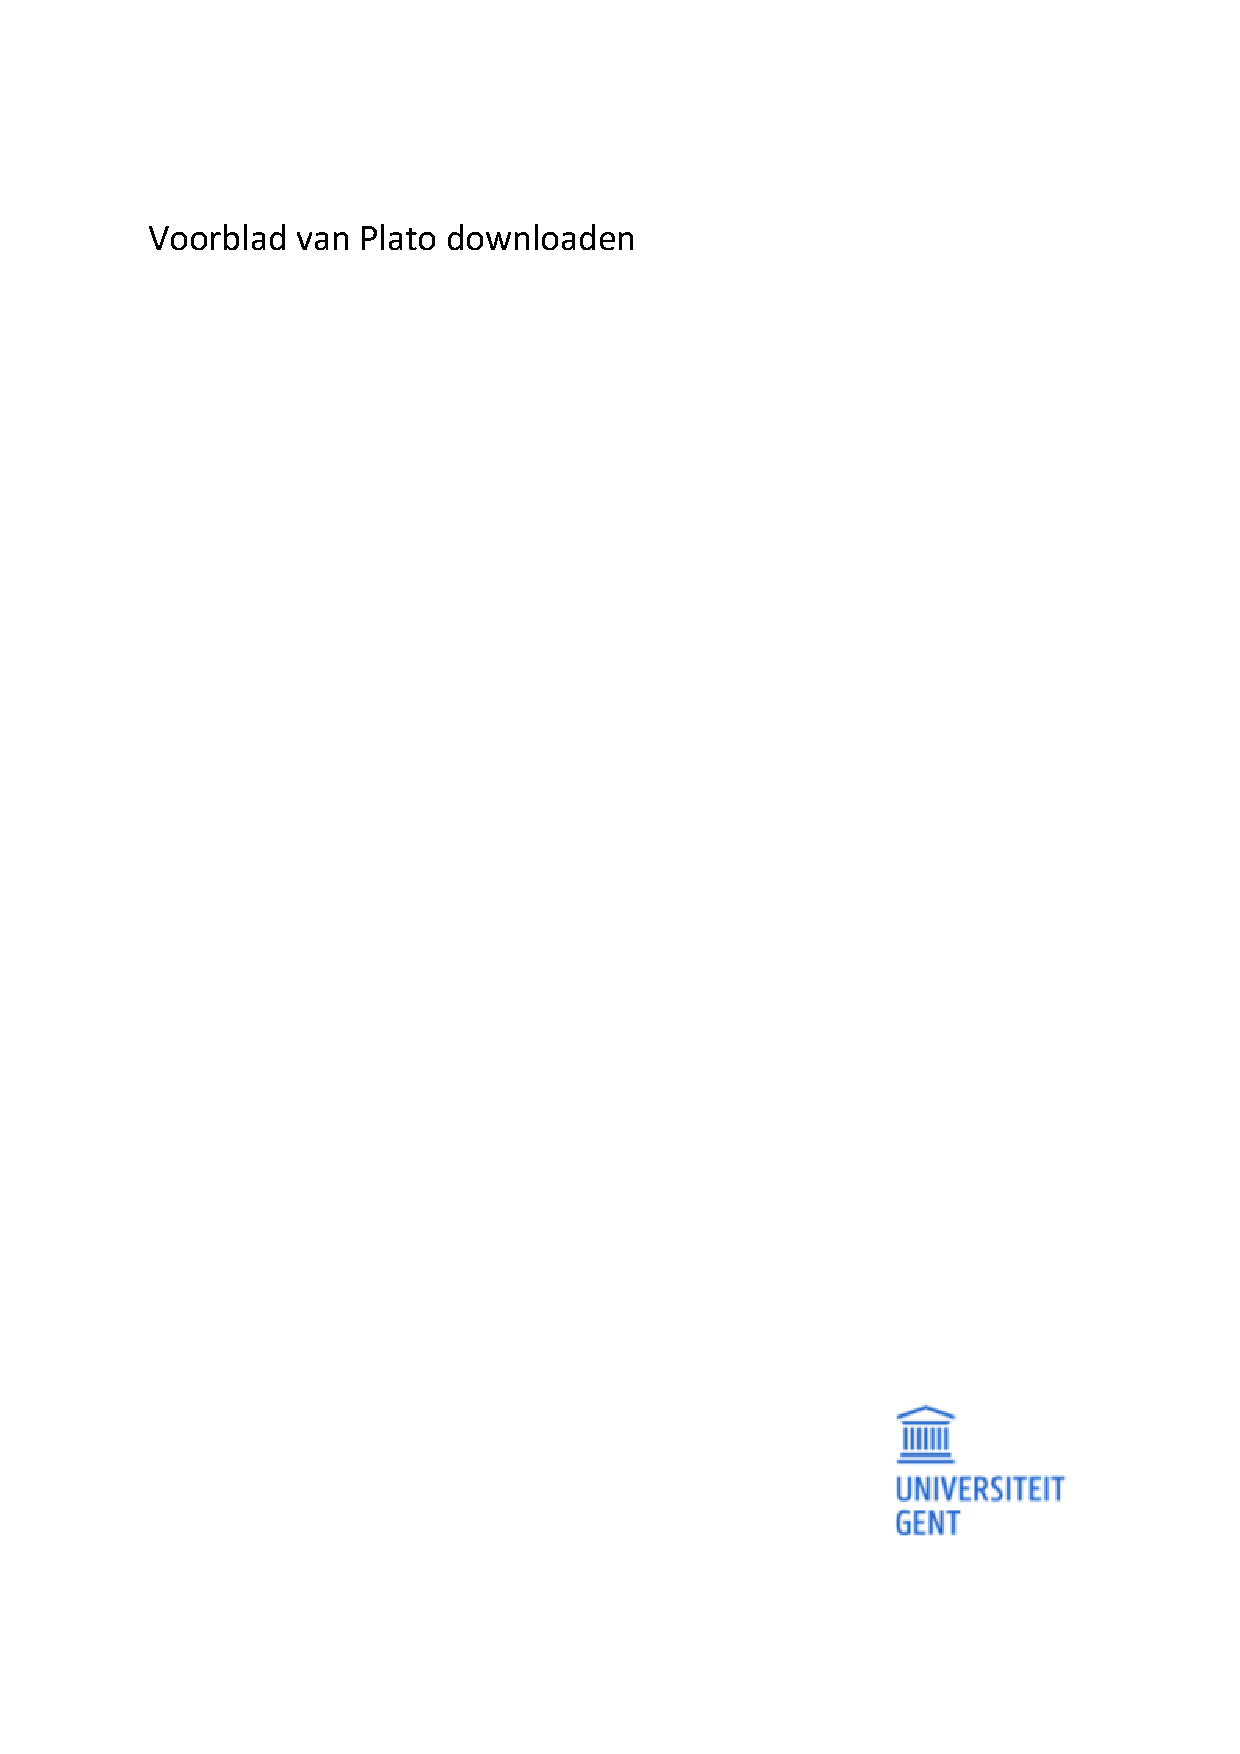
\includepdf{cover-sheet.pdf}

\pagestyle{plainpage}

\chapter*{Acknowledgements}

There are many people I would like to thank for their valuable advice and support over the past months. During those months, I have had the privilege of immersing myself in what has been an entirely new world for me, at the same time collaborating with very talented people. However, the past months have also been challenging. Therefore, a heartfelt thank you to those who have helped me navigate through them, is more than fitting.

First and foremost, I would like to express my sincere gratitude to Bryan-Elliott Tam. Bryan was my counselor throughout the second and third semesters of the academic year, going above and beyond to navigate me through the realm of link traversal. I distinctly recall one of our initial meetings. Bryan had prepared an entire PowerPoint presentation to help me get started with the new approach for my thesis, which we had decided on just the week before. I was able to dive right in. However, what I am most thankful to Bryan for, are his numerous reassuring and encouraging words during the more challenging moments. Especially during the last month, it brought me a great deal of comfort. So, Bryan, from the bottom of my heart: thank you.

Omdat ik met de volgende mensen in het dagelijkse leven steeds in mijn moedertaal communiceer, schakel ik even over naar het Nederlands. Dat doe ik in eerste instantie om Brecht Van de Vyvere te bedanken. Brecht was mijn begeleider tijdens het eerste semester van het academiejaar en heeft me mijn eerste stappen in de wereld van Linked Data helpen zetten. Dat deed hij altijd met veel zorg en de grootste glimlach. Dankjewel, Brecht.

Iemand die ik zeker niet mag en kan vergeten te bedanken, is Olivier Van D'huynslager. Als digitaal hoofd van CoGent heeft Olivier me bijna een volledig jaar lang mee begeleid. Op bijna elke meeting die ik met mijn begeleider hield, was Olivier aanwezig. Hij nam die extra vergaderingen er met de glimlach bij. Bedankt voor al je ideeën en goede raad, Olivier.

Ook Pieter Colpaert wil ik bedanken. Hij was anderhalf jaar geleden degene die me tijdens een wandeling in de Blaarmeersen kennis liet maken met de wereld van Linked Data. Dat deed hij met veel overgave en passie. Ik hoefde dan ook niet lang te twijfelen welk masterproefonderwerp ik zou kiezen. Bedankt, Pieter.

Dan zijn we aangekomen bij mijn familie. Ik ga het mezelf niet te moeilijk maken en meteen met mijn ouders beginnen. Zij zullen namelijk ook gemerkt hebben dat dit laatste jaar voor mij veruit de meest uitdagende van de voorbije zes was. Gelukkig heb ik de beste ouders die iemand zich kan wensen, en stonden zij trouw op de eerste rij om me er met aanmoedigende woorden en veel liefde doorheen te loodsen. Mama en papa, ik zal het jullie nog wel luidop zeggen, maar hier staat het alvast zwart op wit: dankjewel.

Wie ook zeker niet mag ontbreken op deze pagina, zijn mijn grootouders. Niet alleen tijdens het schrijven van mijn masterproef, maar jarenlang, tijdens elke examenperiode, mocht ik bij hen - gewoon het hoekje om - in alle rust komen werken. Elke dag opnieuw werd ik beladen met lekker eten, tussendoortjes, aanmoedigingen en vooral veel liefde. Ik heb veel onvergetelijke momenten meegemaakt tijdens mijn studententijd, maar ik lieg niet als ik zeg dat ik de dagen bij hen nog het meest zal missen. Lieve moemoe en grootva, ik ben jullie eeuwig dankbaar.

En dan is er nog iemand die ongetwijfeld niet kan wachten haar naam te horen. Mijn allerliefste Eva, dankjewel voor al die weken, maanden en jaren onophoudelijke steun. Ik weet niet hoe je het doet, maar zelfs op de moeilijkste momenten slaag je er telkens weer in mij op te rapen en met nieuwe moed vooruit te doen kijken. Ik kan niet wachten om met jou de volgende fase van mijn - ons - leven te beginnen. Ik zie je graag.

Ten slotte wil ik ook alle mensen die ik nog niet vermeld heb maar die me toch al die tijd gesteund hebben, heel oprecht bedanken. Ik denk daarbij aan familie, vrienden, medestudenten ... Die steun hoeft zelfs niet altijd uitgesproken te zijn. Een schouderklopje of een aanmoedigende glimlach kan al een wereld van verschil maken. Het zijn de kleine gebaren die het 'm doen. Dankjewel allemaal!
\chapter*{Toelichting in verband met het masterproefwerk}

Deze masterproef vormt een onderdeel van een examen. Eventuele opmerkingen die door de beoordelingscommissie tijdens de mondelinge uiteenzetting van de masterproef werden geformuleerd, werden niet verwerkt in deze tekst.

% This master's dissertation is part of an exam. Any comments formulated by the assessment committee during the oral presentation of the master's dissertation are not included in this text.

\subsection*{Melding van vertrouwelijkheid (enkel indien van toepassing)}

Bekijk hiervoor de informatie op \href{https://www.ugent.be/ea/nl/faculteit/studentenadministratie/masterproef/} {de facultaire website} - \textbf{Nota in verband met de vorm van de masterproef (alle opleidingen)}
\chapter*{Abstract}
\chaptermark{Abstract}
\addcontentsline{toc}{chapter}{Abstract}

\section*{English}

This master's thesis explores the innovative approach of discovering digital art collections using Link-Traversal-based Querying, focusing on the Collections of Ghent (CoGhent) data. CoGhent, a former partnership that digitized collections from cultural institutions, published the data as Linked Data in RDF format. By employing link traversal, this data can be explored in new ways, offering fresh insights into art collections.

The Comunica platform is central to this process, allowing for link traversal of RDF datasets and enabling the extraction of valuable data. In the CoGhent data, for instance, each entity referred to as a \textit{Human-Made Object}, such as an art piece, links to a IIIF Manifest. This manifest is a JSON-LD document that specifies artwork data and may provide instructions for digital display. Particularly, it holds a link to a picture of the piece, offering a visual representation of the artwork.

However, some resource links in the CoGhent data, notably Getty Vocabularies links, do not return an RDF compliant document, presenting a challenge for the Comunica link traversal engine. Workarounds are needed to reach the RDF compliant counterparts of these non-RDF compliant documents.

To make the discovery of CoGent collections accessible and assist art enthusiasts or professionals without a technical background in constructing SPARQL queries for a link traversal engine, two web application ideas are proposed. The first allows users to select predetermined properties of artworks, accompanied by a question indicating the purpose of the property. Each property corresponds to a sequence of predicates, which the application can ultimately use to generate a query. The second idea enables users to start from a resource of their choice, build a tree of predicates and objects, and eventually select objects of interest for query construction.

Ultimately, the discovered data can be incorporated in a IIIF Manifest, allowing display using a IIIF Viewer. This approach enhances the accessibility of art collections and provides a novel way to explore the rich cultural heritage in the CoGhent data.

\newpage
\newpagestyle{plainpage}{
  \sethead{}{}{}
  \setfoot{}{\thepage}{}
  \setheadrule{0pt}
}
\pagestyle{plainpage}

\section*{Nederlands}

Deze masterproef onderzoekt hoe digitale kunstcollecties met behulp van Link-Traversal-based Querying verkend kunnen worden. De focus ligt daarbij op de data die gepubliceerd werd door de Collectie van de Gentenaar (CoGent). Dit gewezen samenwerkingsverband digitaliseerde collecties van culturele instellingen en publiceerde de gegevens als Linked Data in RDF-formaat. Door link traversal te gebruiken, kunnen deze gegevens op nieuwe manieren worden verkend, wat leidt tot nieuwe inzichten in kunstcollecties.

Het Comunica-platform speelt een centrale rol in dit proces. Het maakt link traversal van RDF-datasets mogelijk, waardoor waardevolle gegevens kunnen worden verkregen. In de CoGent-data, bijvoorbeeld, verwijst elke entiteit die wordt aangeduid als een \textit{Mensgemaakt Object}, zoals een kunstwerk, naar een IIIF Manifest. Dit manifest is een JSON-LD-document dat kunstwerkgegevens specificeert en mogelijk instructies geeft voor digitale weergave. In het bijzonder bevat het een link naar een afbeelding van het stuk.

Echter, sommige resource-links in de CoGent-data, met name Getty Vocabularies-links, geven geen RDF-conform document terug. Hier kan Comunica niet mee aan de slag. Er zijn dus oplossingen nodig om de RDF-conforme tegenhangers te bereiken.

Om de ontdekking van CoGent-collecties toegankelijk te maken en kunstliefhebbers of professionals zonder technische achtergrond te helpen bij het opstellen van SPARQL-queries voor een link traversal engine, worden twee ideeën voor webapplicaties voorgesteld. Het eerste stelt gebruikers in staat om vooraf bepaalde eigenschappen van kunstwerken te selecteren, vergezeld van een vraag die het doel van de eigenschap aangeeft. Elke eigenschap komt overeen met een aaneenschakeling van predicaten, waarmee de applicatie uiteindelijk een query kan genereren. Het tweede idee stelt gebruikers in staat om vanuit een resource naar keuze, een boom van predicates en objecten op te bouwen, en finaal objecten van belang te selecteren voor queryconstructie.

Uiteindelijk kunnen de ontdekte gegevens worden toegewezen aan een IIIF Manifest, waarna een IIIF Viewer ze kan visualiseren. Deze benadering vergroot de toegankelijkheid van kunstcollecties en biedt een nieuwe manier om het rijke culturele erfgoed in de CoGent-data te verkennen.
% Write the extended abstract as a separate project using the IEEE conference proceedings template, and include the resulting PDF here in the document. You can find the template on Overleaf: https://www.overleaf.com/latex/templates/ieee-conference-template/grfzhhncsfqn. 

%Voeg dit toe als .pdf
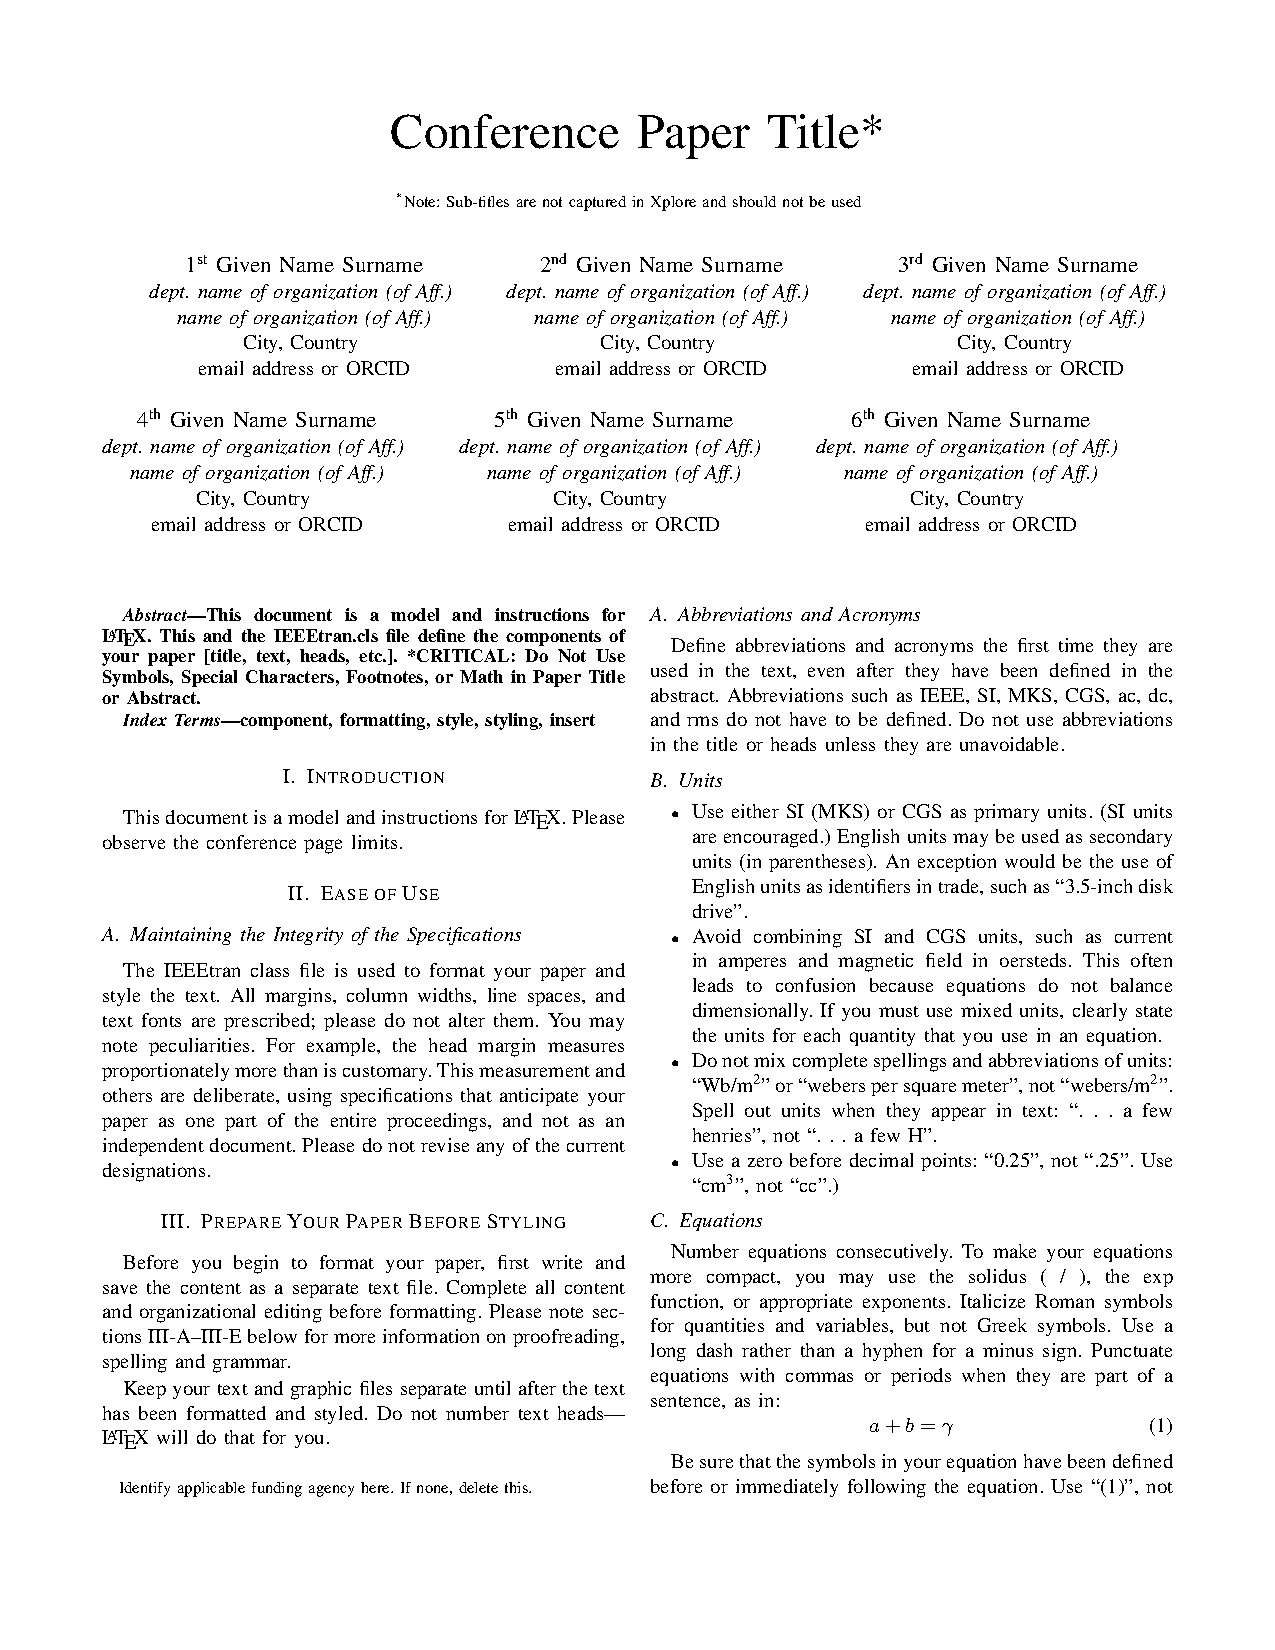
\includepdf[pages={-}]{abstract.pdf}  % Extended Abstract

\tableofcontents\newpage
\listoffigures\newpage
\listoftables\newpage
%%%%%%%%%%%%%%%%%%%%%%%%%%%%%%%%%%%%%%%%%%%%%%%%%%%%%%%%%%%%%%%
%                                                             %
% Note: To add or remove acronyms, modify `personal_data.tex` %
%                                                             %
%%%%%%%%%%%%%%%%%%%%%%%%%%%%%%%%%%%%%%%%%%%%%%%%%%%%%%%%%%%%%%%


% Print the glossary
\printglossary[type=\acronymtype, title={List of Acronyms}]

\glsaddallunused[\acronymtype]                              % make sure all unused acronyms are in list

\setlist[description]{style=standard} % reset list settings back to default

\listoflistings\newpage

%
% Include the main chapters of the thesis below
% Note: it's best to avoid spaces in filenames as Latex might complain about them.
%
\mainmatter
\pagestyle{fancy} % Use header
\chapter*{Introduction}
\chaptermark{Introduction}
\addcontentsline{toc}{chapter}{Introduction}

Digital art collections have long stood as a testament to human creativity and cultural evolution. With the advent of technology, many of these collections have undergone digitization, making them more accessible to a global audience. This digitization not only preserves the integrity of the artworks but also offers an opportunity for deeper exploration and understanding. However, with this digital transformation comes a set of challenges, especially for those without a technical background. Professionals in the cultural domain and general art enthusiasts, while passionate about art, may not possess the technical expertise to navigate and query these digitized datasets. This limitation can hinder their ability to make new discoveries and truly immerse themselves in the digital art world.

Discovering art collections can be interpreted in myriad ways. At its core, discovery is about unearthing new insights, understanding the nuances of each artwork, and drawing connections that might not be immediately apparent. This research primarily focuses on retrieving the inherent properties of cultural objects, delving into the intricate details that make each piece unique. However, the true potential of discovery lies in going beyond the confines of a single dataset. Link traversal offers this opportunity, allowing for a broader exploration that extends beyond the immediate dataset, unveiling new layers of knowledge and understanding.

By employing link traversal, one can uncover hidden relationships, gain a deeper understanding of cultural objects, and even compare different artworks in novel and enlightening ways. This approach is particularly beneficial when exploring the Collections of Ghent (CoGhent), a collaborative initiative between various cultural institutions. Published in a Linked Data format, the CoGhent collections are primed for link traversal, enabling a richer and more comprehensive exploration.

This research situates itself at the intersection of art and technology, aiming to bridge the gap between the two. It seeks to empower both professionals and art enthusiasts to navigate the digital art landscape, harnessing the power of link traversal to make new discoveries and draw meaningful connections. Through a systematic exploration of the Collections of Ghent and the development of tools tailored for query formulation, this research offers a roadmap for discovering digital art collections in their entirety.

Chapter~\ref{chap:rel_work} elucidates the foundational concepts of Linked Data and their real-world applications. It delves into the core principles, data modeling, and various RDF syntaxes, setting the stage for a deeper exploration of link traversal in the subsequent chapters. 

Chapter~\ref{chap:coghent_link_traversal} focuses on the CoGhent collections, highlighting the potential of link traversal for discovering properties of Human-Made Objects. It provides an overview of the available data sources and the development of a link traversal engine optimized for the objectives of this research.

In Chapter~\ref{chap:tools_query_building}, the emphasis shifts to the development of user-centric tools for query formulation. Two conceptual web applications are introduced, designed to alleviate the technical complexities of query formulation for users. The chapter also discusses the fundamental functionality shared by both web applications, ensuring a cohesive exploration throughout.

Lastly, Chapter~\ref{chap:handling_query_results} addresses the challenges of visualizing and preserving query results. It offers an overview of potential solutions, outlining their advantages and drawbacks, ensuring that the treasures within the CoGhent collections are accessible and meaningful to all.
\chapter{Titel van het tweede hoofdstuk}
\label{chap:rel_work}

In dit hoofdstuk ...

\section{Sectie titel 1}
\label{sec:related_work}
Vul aan ...
\section{Sectie titel 2}
Vul aan ...
\chapter{Titel derde hoofdstuk}
\label{chap:evaluation}

In dit hoofdstuk ...

\section{Sectie titel}
\label{sec:scalable_faafo}

Vul aan...

\chapter{Titel vierde hoofdstuk}

In dit hoofdstuk ...

\section{Sectie titel}

Vul aan ...

\section{Sectie titel2}

Vul aan ...

\subsection{Subtitel}
Vul aan ...
\chapter*{Conclusie}
\chaptermark{Conclusie}
\addcontentsline{toc}{chapter}{Conclusie}  

Vul aan...

\phantomsection
\section*{Ethische en maatschappelijke reflectie}
\addcontentsline{toc}{section}{Ethische en maatschappelijke reflectie}  

Deze sectie is enkel vereist voor de opleidingen industrieel ingenieur. De locatie van deze sectie lichtjes af van de volgorde voorgeschreven door de faculteit. Wij raden aan om deze reflectie als deel van de conclusie te maken omdat je daardoor eenvoudig kan refereren naar resultaten in je masterproef zelf.

Meer informatie kan je opzoeken op https://www.sdgs.be/nl/sdgs




\renewcommand\bibname{Referenties}
\bibliography{referenties}


\pagestyle{numberless} 
\pagestyle{empty}
\begin{appendices}
\section*{Bijlage A}
\addcontentsline{toc}{section}{Bijlage A}  

Toelichting bijlage.



\newpage
\section*{Bijlage B}
\addcontentsline{toc}{section}{Bijlage B}  

Toelichting bijlage.

\end{appendices}


\end{document}
